\section{malloc实现}\label{sec:malloc实现}

\begin{frame}[fragile]{一些问题?}
    \begin{itemize}[<+- | alert@+>]
        \item 能不能 free() 一部分, 比如 malloc() 得到的 ptr, \texttt{free(ptr + 1)}?
        \item 能不能 free() 不是 malloc() 得到的指针?
        \item 能不能 free() 同一个指针两次?
        \item 好像越界一点点没问题?
        \item 需要知道一些 malloc() 实现的细节!
        \item 点击下载 \href{http://problemoverflow.top/download/my\_malloc.zip}{my\_malloc.zip}
    \end{itemize}
\end{frame}

\begin{frame}[fragile]{malloc实现细节}
    链表.
\end{frame}

\begin{frame}[fragile]{malloc实现细节}
    malloc():
    \begin{itemize}[<+- | alert@+>]
        \item 从双向链表 free\_list 中找到一个合适大小的 chunk
        \item 找不到就向系统申请一块空间, 将多申请的空间放入 free\_list 中, 返回申请到的内存的某个位置的指针
        \item 找到了, 先看 chunk 能不能拆分, 能拆就取一部分出来返回(以节约内存), 不能拆就把整个 chunk 返回
    \end{itemize}
    free():
    \begin{itemize}[<+- | alert@+>]
        \item 如果参数 ptr 不为NULL, 则将 ptr 放回 free\_list 以回收利用
        \item 如果放回后有 chunk 能合并, 则合并以减少内存碎片化
    \end{itemize}
\end{frame}

\begin{frame}[fragile]{free\_list}
    \scriptsize\begin{verbatim}
struct my_malloc_chunk {
    size_t unused;
    size_t size;
    struct my_malloc_chunk *previous;
    struct my_malloc_chunk *next;
} *free_list;
    \end{verbatim}
    free\_list 为类型为 my\_malloc\_chunk* 的链表头指针, 为 NULL 表示没有分配的内存
    \begin{figure}[ht!]
        \centering
        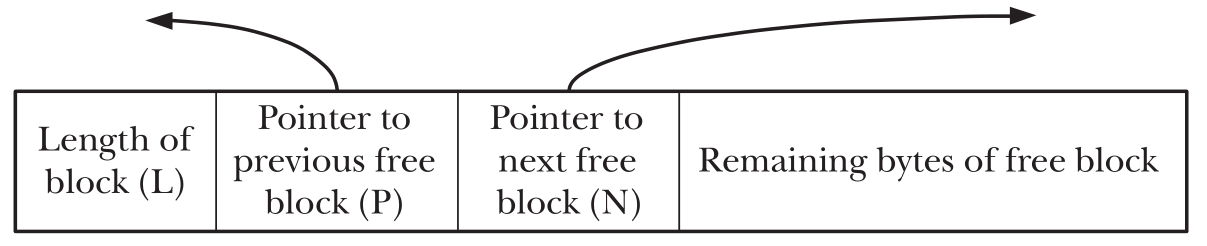
\includegraphics[width=60mm]{figs/my_malloc_chunk.png}
        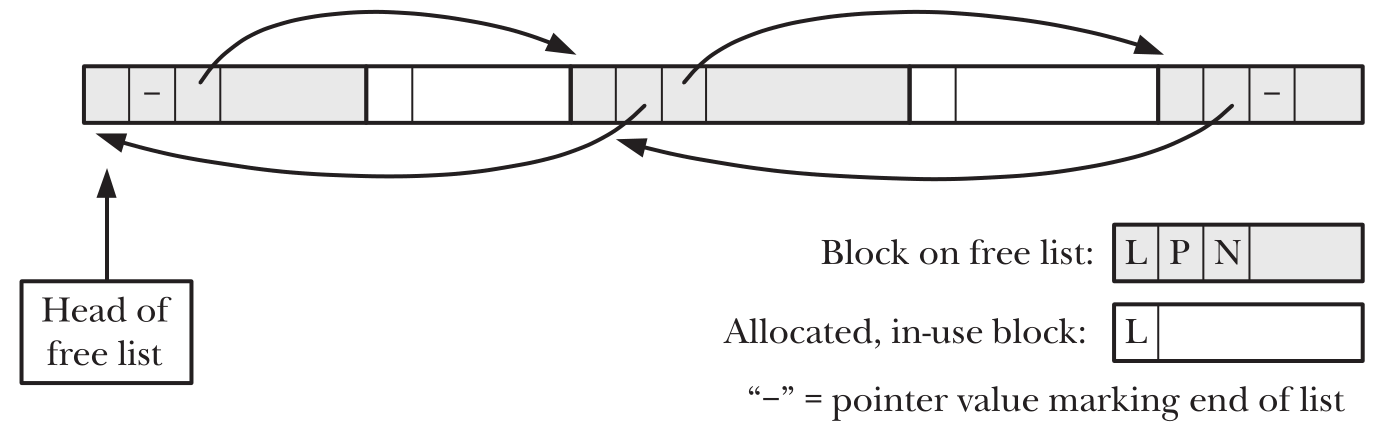
\includegraphics[width=80mm]{figs/free_list.png}
        \caption{free\_list}
    \end{figure}
\end{frame}

\begin{frame}[fragile]{向系统申请空间}
    \begin{itemize}[<+- | alert@+>]
        \item 程序能申请增大或减小堆空间大小
        \item 堆位于未初始化数据区域, 当前的限制称为 program break (可以理解为一个指针)
        \item 增加或减小堆大小, 系统只要相应地提升或降低 program break 指向位置即可
        \item brk() 和 sbrk() 系统调用用来做这件事
    \end{itemize}
\end{frame}

\begin{frame}[fragile]{向系统申请空间}
    \small\begin{verbatim}
#include <unistd.h>

int brk(void * end_data_segment);
    // Returns 0 on success, or –1 on error

void *sbrk(intptr_t increment);
    // Returns previous program break on success,
    // or (void *) –1 on error
    \end{verbatim}
\end{frame}

\begin{frame}[fragile]{malloc实验教程}
    \begin{itemize}[<+- | alert@+>]
        \item 下载 \href{http://problemoverflow.top/download/my\_malloc.zip}{my\_malloc.zip}
        \item 编译运行test, 程序使用的标准库 malloc()
        \item 在 test.c 中找到并取消注释 \texttt{//\#define USE\_MY\_MALLOC}
        \item 如果你使用的 Linux 环境或 Cygwin, 可以注释掉 \texttt{\#define NOT\_UNIX} (在 my\_malloc.h)
        \item 编译运行test, 程序给出提示并异常退出
        \item TODO: 你需要在 my\_malloc.c 文件实现 allocate\_more\_chunk() 相关代码
    \end{itemize}
\end{frame}

\begin{frame}[fragile]{malloc实验教程}
    \begin{itemize}[<+- | alert@+>]
        \item 编译运行test, 程序正常执行, 对比使用标准库 malloc() 的输出
        \item 我们的程序使用了很大的内存
        \item 原因是从 free\_list 删除一个结点时直接把 free\_list 赋为 NULL, 已申请的空间全部不能回收利用
        \item TODO: 实现 delete\_from\_free() 相关代码
    \end{itemize}
\end{frame}

\begin{frame}[fragile]{malloc实验教程}
    \begin{itemize}[<+- | alert@+>]
        \item 编译运行test, 程序用的内存减少, 但仍然很多
        \item 程序没有对大块的内存进行切分
        \item TODO: 实现 get\_pointer() 相关代码
    \end{itemize}
\end{frame}

\begin{frame}[fragile]{malloc实验教程}
    \begin{itemize}[<+- | alert@+>]
        \item 编译运行test, 根据你实现的不同, 程序运行起来可能超级慢! 而且内存使用不降反增!
        \item 对内存切分造成了许多小的内存碎片, 这些碎片难以分配出去且使得链表变长
        \item 搜索 chunk 时如果有刚好相同或差不多大小的 chunk, 切分时可减少内存碎片
        \item TODO: 实现 find\_fit\_chunk() 相关代码, 使用best-fit搜索策略
    \end{itemize}
\end{frame}

\begin{frame}[fragile]{malloc实验教程}
    \begin{itemize}[<+- | alert@+>]
        \item 编译运行test, 程序变快了, 内存使用也减少了, 但运行仍然太慢
        \item 内存碎片仍没有得到有效解决, 代码只切分 chunk 而很少合并
        \item TODO: 实现 add\_to\_free() 相关代码, 改进加入链表和合并策略
    \end{itemize}
\end{frame}

\begin{frame}[fragile]{malloc实验教程}
    \begin{itemize}[<+- | alert@+>]
        \item 编译运行test, 程序又变快了很多, 内存使用量也变得稳定, 虽然运行速度仍远远比不上标准库
        \item 还有什么可以改进的地方?
        \item 机器对地址对齐的数据处理较快
        \item TODO: 实现 request\_size() 相关代码, 满足对齐要求
    \end{itemize}
\end{frame}

\begin{frame}[fragile]{malloc实验教程}
    \begin{itemize}[<+- | alert@+>]
        \item 编译运行test, 速度只得到了小幅改进
        \item 还有什么可以改进的地方?
        \item 编译gprof, 查看函数调用执行时间和占比, 进一步优化你的程序
        \item 更多可实现的地方请参看源代码 TODO advanced
    \end{itemize}
\end{frame}

\begin{frame}[fragile]{一些问题还有吗?}
    \begin{itemize}[<+- | alert@+>]
        \item 能不能 free() 一部分, 比如 malloc() 得到的 ptr, \texttt{free(ptr + 1)}?
        \item 能不能 free() 不是 malloc() 得到的指针?
        \item 能不能 free() 同一个指针两次?
        \item 好像越界一点点没问题?
    \end{itemize}
\end{frame}

\begin{frame}[fragile]{更多资料}
    \begin{itemize}[<+- | alert@+>]
        \item 较好的Linux系统编程书籍: \href{http://www.man7.org/tlpi/toc-detailed.html#ch_7}{tlpi ch7: MEMORY ALLOCATION}
        \item 维基百科: \href{https://en.wikipedia.org/wiki/C_dynamic_memory_allocation}{C dynamic memory allocation}
        \item 完全使用 mmap() 实现的 malloc(): \href{https://code.woboq.org/userspace/glibc/malloc/tst-interpose-aux.c.html}{tst-interpose-aux.c}
        \item 最详细的 glibc 官方文档: \href{http://www.gnu.org/software/libc/manual/html_mono/libc.html#Memory-Allocation}{Memory-Allocation}
    \end{itemize}
\end{frame}